% Einstellungen
% =============

% Da die Einstellungen sich von Dokument zu Dokument kaum verändern,
% ist es sinnvoll, diese an einer zentralen Stelle abzulegen und von
% dort zu laden. Dies geschieht völlig transparent mit dem Befehl
% \input{<Pfad>}, dem als Argument eine Datei mit (relativem) Zugriffs-
% pfad übergeben wird
%23456789012345678901234567890123456789012345678901234567890123456789012
\wlog{This is twp-cfg, the common configuration file all documents
  (JHf)}

% Einstellungen werden in LaTeX vor allen Dingen durch das Einbinden
% von Paketen vorgenommen:
% \usepackage[parameter]{package}

\usepackage{iftex}              % Test des Formatierers, durch \if...
                                % können Anpassungen an den Prozessor
                                % vorgenommen werden
\ifluatex                       % wenn mit dem neuen TeX-Prozessor,
                                % der mehr Fontarten unterstützt,
                                % gearbeitet wird:
                                % - pk-Fonts (Pixelfonts, nicht
                                %   skalierbar, alt)
                                % - pfb-Fonts (Fonts, die durch Kurven
                                %   beschrieben werden, skalierbar,
                                %   entwickelt von Adobe->Acrobat
                                %   Reader)
                                % - otf/ttf-Fonts (Fonts, die durch
                                %   Kurven beschrieben werden,
                                %   skalierbar, entwickelt von Apple
                                %   und Microsoft, um Adobe-Lizenzen
                                %   zu sparen)
  %---- Eingabezeichensatz --------------------------------------------
                                % luatex unterstützt utf-8, also keine
                                % Festlegung des Eingabezeichensatzes
                                % erforderlich
  %---- Grundfont -----------------------------------------------------
  \usepackage{fontspec}         % Festlegen der Fontverwaltung für
                                % LuaTeX.
  \defaultfontfeatures{Renderer=Basic, Ligatures=TeX}
  \fontspec{Latin Modern Roman}
  \setmonofont[Scale=0.85]{Luxi Mono Regular} % muss aktiviert werden,
                                % falls das Paket installiert ist
\else
  %---- Eingabezeichensatz --------------------------------------------
  \usepackage[utf8]{inputenc}   % Eingabe deutscher Umlaute
                                % Unix/Linux: utf8
                                % Unix/Linux: latin1 (alt)
                                % Windows: cp1250
  %---- Grundfont -----------------------------------------------------
  \usepackage[T1]{fontenc}      % ec-Fonts
  \usepackage{lmodern}          % wg. der lm-Fonts (keine bitmap-Fonts!)
\fi

%---- Sprachauswahl ---------------------------------------------------
\usepackage{babel}              % um deutsche Bezeichnungen benutzen
                                % zu können, es wird der Parameter aus
                                % dem Kopf des Dokumentes benutzt.

%---- Verwaltung der Bibliographie, muss nach babel geladen werden ----
                                % Verwaltung der
                                % Bibliographie durch
\usepackage[backend=biber,      % Biber und biblatex
            autolang=other,     % Trennung gemäß der mit
                                % babel gesetzten Sprache
            style=alphabetic,   % Verweise ähnlich zu
                                % alpha.bst: XXX00
            citestyle=alphabetic, % mehrere Titel eines
                                % Autors werden XXX00a,
                                % XXX00b, ... zitiert
            giveninits=false,   % Vornamen werden nicht
                                % abgekürzt
            ]{biblatex}
\usepackage[babel,german=quotes]{csquotes} % Titel werden
                                % in deutsche Gänsefüßchen
                                % gesetzt
\addbibresource{../../shared/latex_course.bib}   % muss mit
                                % .bib-Datenbanken gefüllt werden
\ifluatex\else
  \usepackage{babelbib}         % fuer eine dazu passende Bibliographie,
                                % luatex kennt seine eigene
                                % Bibliographieverwaltung
\fi
\defbibheading{bibliography}[Literaturverzeichnis]{\chapter*{#1}}

%---- Sonstiges ------------------------------------------------------
% \PassOptionsToPackage{debugshow,final}{graphicx} % bei Bedarf zu
                                % aktivieren
\usepackage{graphicx}           % Vorbereitung der Graphiken
% \graphicspath{{...}{...}}     % muss mit entsprechenden Pfaden
                                % gefüllt werden, hier
\graphicspath{%                 % weitere Pfade können nach dem
  {../../shared/figures}%       % gleichen Muster hinzugefügt werden
}
\usepackage{listings}           % zur Darstellung von Code aller Art
\lstset{                        % Einstellungen des listings-Paketes
  language=tex,                 % es wird TeX\LaTeX-Code formatiert
  style=colored,                % der Hintergrund und spezielle Befehle
                                % werden farbig dargestellt,
  escapechar=@,                 % mit dem @-Zeichen gibt es die
                                % Möglichkeit,
                                % "ausgezeichneten" Text zu zeigen
}
%\usepackage{isodate}            % wg. \printdate{date}
\usepackage{booktabs}           % wg. \toprule, ...
                                % für typografisch korrekte Linien
\usepackage{moreverb}           % zum Schreiben von Texten in externe
                                % Dateien
\usepackage{tikz}               % TikZ ist kein Zeichenprogramm
\usetikzlibrary{trees}          % Produzieren von Baumstrukturen

\usepackage{pgfplots}           % Darstellung von Funktionen
\pgfplotsset{width=7cm,compat=1.18} % Standardbreite und Kompatibilitätslevel

\usepackage{amsmath}            % für die einfachere Eingabe math. Gleichungen,
                                % muss/sollte als Standard genutzt werden
\usepackage{rotating}           % für die nicht horizontale Textausrichtung
\usepackage{xspace}             % \wg. \xspace: fügt ein Leerzeichen an einen
                                % Text an, außer der Text ist von einem
                                % Punktuationszeichen gefolgt

                                % die nächsten Pakete dienen der Einstellung
                                % von Kopf- und Fußzeile
\usepackage[useregional]{datetime2}  % das Paket zur Darstellung von Tag und
                                % Uhrzeit in einem Format, das im deutschen
                                % Sprachbereich üblich ist
%\renewcommand{\dateseparator}{.}% das übliche Trennzeichen
\newsavebox{\NameAndDate}       % Name und Datum werden nur einmal bestimmt
                                % und dann zum späteren Gebrauch gespeichert
\usepackage[headsepline, footsepline]{scrlayer-scrpage} % das ist das
                                % eigentliche Paket, wir wollen Kopf- und
                                % Fußzeile durch Linien abtrennen

\pagestyle{scrheadings}         % das schaltet das neue Seitenlayout ein
\setkomafont{pagehead}{\normalfont\bfseries} % die Kopfzeile fett
\ifoot{\usebox{\NameAndDate}}   % Name und Datum innen auf der Seite
\AtBeginDocument{%              % wenn \begin{document} erreicht wird,
  \sbox{\NameAndDate}{%
    \footnotesize\textsf{%
      N.~N.: Meine eigene Probearbeit, \today--\DTMcurrenttime%
    }
  }
}

\usepackage{ifthen}             % zur Unterstützung logischer Bedingungen

%---- Bezuege --------------------------------------------------------
% gemäß der cleveref Dokumentation müssen diese Pakete als letzte
% geladen werden
\usepackage{varioref}           % Voraussetzung für cleveref
\usepackage[ngerman]{cleveref}  % deutschsprachige Bezuege, nach babel
                                % zu laden

%---- Einstellungen ---------------------------------------------------
\setcounter{secnumdepth}{7}     % Anzeige der Gliederungsstufen bis
                                % hinunter auf Ebene 7
\setcounter{tocdepth}{7}        % Inhaltsverzeichnis zeigt
                                % Gliederungsstufen bis
                                % hinunter auf Ebene 7, gebraucht wird
                                % das höchstens für technische
                                % Dokumentationen
\newlength{\myWidth}            % universelle Längenangabe, die
                                % jeweils passen gesetzt wird

%---- Eigene Definitionen ---------------------------------------------
\author{Jobst Hoffmann}
\title{Ein erstes \LaTeX-Dokument mit der Dokumentklasse
\texttt{scrartcl}}       % \texttt{<Inhalt>} formatiert <Inhalt>
                         % mit einer dicktengleichen Schriftart

% Hier werden nun eigene Befehle definiert, eine genaue Anleitung
% zur Definition eigener Befehle folgt später:
% \cs:    command sequence, das Argument wird als Befehl formatiert
\NewDocumentCommand{\cs}{m}{\texttt{\char92#1}}
% \farg:  fixed argument, das Argument wird als festes Argument eines
%        Befehls formatiert
\NewDocumentCommand{\farg}{m}
{%
  {\texttt{\{#1\}}}%
}
% \farg:  fixed optional argument, das Argument wird als optionales
%         Argument eines Befehls formatiert
\NewDocumentCommand{\foarg}{m}
{%
  {\texttt{[#1]}}%
}
% \marg:  mandatory argument, das Argument wird als verpflichtendes,
%         aber frei zu wählendes Argument eines Befehls formatiert
\NewDocumentCommand{\marg}{m}
{%
  {\texttt{\{}\(\langle\)\textit{#1}\(\rangle\)\texttt{\}}}%
}
% \meta:  das Argument wird als Beschreibung eines Objektes benutzt
\NewDocumentCommand{\meta}{m}
{%
  {\ensuremath{\langle}\textit{#1}\ensuremath{\rangle}}%
}
% \oarg:  optional argument, das Argument wird als optionales,
%         frei zu wählendes Argument eines Befehls formatiert
\NewDocumentCommand{\oarg}{m}
{%
  {\texttt{[}\(\langle\)\textit{#1}\(\rangle\)\texttt{]}}%
}
% \Cee: der Buchstabe C als Name der Programmiersprache,
%       \xspace sorgt dafür, dass das Kommando bei Bedarf
%       mit einem Leerzeichen ergänzt wird
\NewDocumentCommand{\Cee}{}{\textsc{C}\xspace}

% in dieser Datei werden alle Zusatzpakete mittels
% \usepackage{<package>} geladen


% merke: ein späterer Titel überschreibt einen früher gesetzten Titel,
% in der scrreprt-Dokumentenklasse erscheint der Titel auf einer
% eigenen Seite
\title{Ein erstes \LaTeX-Dokument mit der Dokumentklasse \texttt{scrreprt}}
                         % \texttt{<Inhalt>} formatiert <Inhalt>
                         % mit einer dicktengleichen Schriftart
                         % im Vergleich zur ansonsten eingesetzten
                         % Proportionalschrift

% Rumpf des Dokumentes
\begin{document}
\frontmatter                    % es wird mit kleinen, römischen Zahlen
                                % gezählt 

% \maketitle                    % die automatisch erzeugte
                                % Titelseite, dies erfordert
                                % die Angabe des Autors und des
                                % Titels in den Einstellungen,
                                % kann für eine Bachelor-, ...
                                % Arbeir nicht benutzt werden!

\makeatletter
\@ifclassloaded{scrartcl}{
  \maketitle{}
}{
% die selbst entworfene Titelseite, die evtl.
% automatisch angepasst werden kann
\begin{titlepage}

% die Leerzeilen bedeuten immer das Ende bzw. den Beginn eines neuen Absatzes,
% ohne eine Leerzeile wird der laufende Text fortgesetzt

% die Ortsangabe soll einheitlich rechtsbündig gesetzt werden, dafür wird
% die Angabe in einen Kasten
% (\parbox[position][height][inner position]{width}{text}) gepackt, der
% passend verschoben wird

% die Box soll rechtsbündig erscheinen, um waagerechten Leerraum zu erhalten,
% benutzt man \hspace{length}. length kann eine variable Größe ein, mit der
% Platz aufgefüllt wird: \fill

% eine geratene Größe für eine Breite ist manchmal ausreichend, meistens
% aber nicht
\settowidth{\myWidth}{\sffamily\large Angewandte Mathematik und Informatik}
%                     ^ die Auswahl und die Größe des Fonts sind wichtig,
%                       sonst stimmen Größen nicht überein
\hspace{\fill}\parbox{\myWidth}{
  % da mehrere Zeilen in einem anderen Font gesetzt werden sollen, benutzt
  % man Befehle, die gruppenintern gelten
  % \scshape        % Kapitälchen (sc: small caps), alle Buchstaben werden
                    % groß geschrieben, die Großbuchstaben ein bisschen
                    % größer, entspricht nicht dem Corporate Design der FH
  \sffamily         % serifenloser Font
  \raggedleft       % rechtsbündiger Satz
  \large
  Fachhochschule Aachen Campus Jülich

  Medizintechnik und Technomathematik

  Angewandte Mathematik und Informatik
}

% eine gute Einteilung von Titelseiten erfolgt nach dem Drittelprinzip
% oder nach dem Golgenen Schnitt
% Drittelprinzip (um 90° gedreht):
%     2/3      1/3
% +----------+-----+
% |          -     |
% +----------+-----+
%
% Goldener Schnitt (um 90° gedreht):
%       a       b
% +----------+-----+
% |          -     |
% +----------+-----+
%    a:b = (a+b):a
%

\vspace{80pt}
\rule{\textwidth}{2pt}

\begin{center}
\Huge \textsf{\bfseries Meine eigene Probearbeit}

% um senkrechten Leerraum zu erhalten, beginnt man den Absatz mit
% einem \vspace{length}. length ist eine Größe, die in einer
% beliebigen Einheit angegeben werden kann, normalerweise in pt
% pt: point, 1 pt ist der 1/72,27 Teil eines inches (1 in = 2,54 cm),
% 10 pt entsprechen ungefähr 3 mm.
\vspace{20pt}
\Large Bachelorarbeit von N.~N.      % ~: bedeutet einen nicht umbrechbaren
                              %     Zwischenraum, das Fehlen dieses
                              %     Zwischenraumes wäre ein schwerer
                              %     typographischer Fehler, ...
                              % N.~N.: aus dem Lateinischen
                              %     - nomen nominandum: ein noch zu
                              %       benennender Name
                              %     - nomen nescio: ich weiß den Namen
                              %       (noch) nicht
\end{center}

  \rule{\textwidth}{2pt}

\vspace{15pt}
\begin{center}
 Jülich, Dezember 2022
\end{center}

\end{titlepage}
}
\makeatother % die selbst entworfene Titelseite

% Die Zusammenfassung erscheint auf einer eigenen Seite
%\begin{abstract}                % die abstract-Umgebung gibt es
                                % nur in der scrartcl-Klasse!
    Hier steht eine kurze Zusammenfassung des Inhaltes, es geht hier um den
    Aufbau eines Artikels, insbesondere um die geeignete Gliederung.
%\end{abstract}

\tableofcontents

% die Gliederung erfolgt in bis zu 7 Ebenen, abhängig von der Klasse
%   Ebene     Klasse                   Befehl (einfachen Form)
%   0.        scrbook/scrreprt         \chapter{<Titel>}
%   1.        alle                     \section{<Titel>}
%   2.        alle                     \subsection{<Titel>}
%   3.        alle                     \subsubsection{<Titel>}
%   4.        alle                     \paragraph{<Titel>}
%   5.        alle                     \subparagraph{<Titel>}
%   6.        alle, nicht im Original  \subsubparagraph{<Titel>}


\mainmatter                     % Umschaltung auf arabische Ziffern

\chapter{Einleitung}   % Einleitung, Hauptteil und Schluss
                       % dürfen niemals in der fertigen Arbeit
                       % stehen, da muss die Autorin bzw. der Autor
                       % sich etwas Passendes einfallen lassen.

Hier steht der Inhalt des Dokumentes, weiteres siehe im n\"achsten
Beispiel. Der erste Absatz wird ohne Einzug formatiert, wenn er einer \"Uberschrift folgt.

Weitere Absätze bekommen einen Einzug, wie hier deutlich zu sehen ist.
Das soll an dieser Stelle reichen.

In dieser Arbeit wird gezeigt, wie man mit \LaTeX{} arbeitet. Dazu
wird in \cref{chap:TeX} auf die Struktur eines wissenschaftlichen
Dokumentes eingegangen, dabei wird ein spezieller Augenmerk auf die
Befehlsstruktur von \LaTeX{} gerichtet (\cref{sec:befehlsstruktur}).


\chapter{Arbeiten mit \TeX/\LaTeX}% durch dieses %-Zeichen wird
\label{chap:TeX}                  % Leerraum vermeiden, der zu einer
                                  % falschen Nummerierung führen kann
                                  % \label: setzt eine Marke,
                                  % auf die ich mich an andere Stelle
                                  % beziehen kann.

In dieser kleinen Einführung wird beschrieben, wie man mit \LaTeX{} arbeitet.
\LaTeX{} ist ein Makropaket, das von Leslie Lamport auf der Basis 
von \TeX{} \cite{knuth_86:tex_book} entwickelt worden ist. Die aktuelle
Entwicklung geschieht durch "`The \LaTeX{} project"', sie ist im Internet
unter zu verfolgen.

% eine Kurzform der Überschrift, die für das Inhaltsverzeichnis
% geeignet ist erzeugt man mit einem optionalen Argument
\section[Die Befehlsstruktur]{Die Befehlsstruktur von \TeX/\LaTeX}%
\label{sec:befehlsstruktur}

% die Nummerierung wird automatisch korekt erzeugt, wenn die
% Gliederung korrekt ist, eine fehlerhafte Gliederung wird durch 0.
% in der Überschrift angezeigt. Für die Hausaufgaben ist eine
% fehlerhafte Nummerierung ein Ausschlusskriterium
\subsection{\TeX: Einfache Befehle -- Primitive} % das doppelte
           % Minuszeichen
           % ist der sogenannte n-dash, es wird immer dann eingesetzt,
           % wenn ein _deutscher_ Gedankenstrich gebraucht wird

Jedes Zeichen ist ein einfacher Befehl: setze das Zeichen in der
aktuellen Schriftart und der aktuellen Größe an die aktuelle
Position, verändere die aktuelle Position um die Breite des Zeichens.
Es gibt aber Zeichen, die eine besondere Bedeutung haben. Wenn man
diese im Text benötigt, muss man eine Ersatzdarstellung benutzen. Im
Regelfall ist es ein vorweggestellter Gegen-/Rückwärtsschrägstrich
(backslash).
\begin{itemize}                 % Listenumgebungen werden später behandelt
  \item Das \%-Zeichen leitet Kommentar ein.
  \item Das \$-Zeichen leitet in \TeX den einfachen Mathematikmodus ein und
    aus.
  \item Das \(\backslash\)-Zeichen leitet Befehle ein, der Befehl endet mit
    dem ersten Nichtbuchstaben. Wird nach einem Befehl ein Leerzeichen
    benötigt, muss man dieses entweder durch einen weiteres
    \(\backslash\)-Zeichen gefolgt von einem Leerzeichen oder durch ein
    Paar von Gruppenklammern erzeugen: Vergleiche \LaTeX und \LaTeX\ und
    \LaTeX{} und auch \LaTeX.
  \item Geschweifte Klammern (\{ und \}) definieren Gruppen. Dinge, die in
    einer Gruppe definiert sind, sind außerhalb der Gruppe unbekannt.
  \item Das Doppelkreuz \# beschreibt Parameter.
  \item Das kaufmännische Und (\&) wird für das Setzen von Tabellen
    gebraucht.
  \item Der Unterstrich (\_) leitet einen Index ein, gilt nur im
    Mathematikmodus.
  \item Das Dach (\^{}) leitet eine Potenz ein, gilt nur im
    Mathematikmodus.
  \item Die Tilde (\~{}) stellt einen Leerraum dar, der nicht umgebrochen
    werden kann.
\end{itemize}

\subsection{\LaTeX: Einfache Befehle}

\LaTeX{} hat die Befehlsstruktur von \TeX{} übernommen, es gibt bei vielen
Befehlen wie bei den Gliederungsbefehlen optionale Parameter, die sich auf
die Ausführung/Darstellung auswirken. Ein einfacher Befehl hat damit die
Syntax
\begin{lstlisting}[style=colored]
@\cs{\meta{Kommandoname}}\oarg{opt. Parameter}\marg{verpflichtende Parameter}@
\end{lstlisting}

Zusätzlich hat \LaTeX{} den Begriff der Umgebung eingeführt: In einer
Umgebung gibt es zusätzliche Kommandos, die außerhalb der Umgebung
unbekannt sind. Auch eine Umgebung kann optionale Parameter benutzen, diese
werden an das einführende Kommando in eckigen Klammern angehängt.
\begin{lstlisting}
\begin{@\meta{Umgebungsame}@}@\oarg{Optionen}@
    ...
\end{@\meta{Umgebungsame}@}
\end{lstlisting}


\subsection{Gliederung/Strukturierung eines Dokumentes}

Ein wissenschaftliche Arbeit zeichnet sich durch ein paar Dinge aus:
\begin{enumerate}
  \item Eine Gliederung entsprechend dem hier vorliegenden Vorbild.

    Diese wird benutzt, um dem Leser den Überblick über den Inhalt und
    das Verständnis des Inhaltes zu erleichtern. Mit einer Gliederung
    kann man den Leser auf wichtige Dinge vorbereiten, man kann auch
    Rückverweise geben.

    Dies geschieht mit den Kommandos
    \lstinline[mathescape]|\label{$\meta{Marke}$}| und
    \lstinline[mathescape]|\cref{$\meta{Marke}$}|. Dabei muss Marke in
    beiden Fällen identisch sein, ein Tippfehler führt zu
    Fehlermeldungen, im Text erscheint \textbf{??}, um den Fehler
    sichtbar zu machen.

\end{enumerate}



\subsection{Weitere Untergliederung Teil 4}

Hier wird gezeigt, wie man auf das Inhaltsverzeichnis und die
Nummerierung der Unterabschnitte Einfluss nehmen kann. Standarmäßig
wird nummeriert bis zur \lstinline|\subsection|, wenn weitergehend
nummeriert werden soll, muss man entsprechende Grenzen setzen
\begin{lstlisting}
  \setcounter{secnumdepth}@\marg{Tiefe}@
\end{lstlisting}
\meta{Tiefe} gibt die Stufe an, bis zu der nummeriert werden soll.

\subsubsection{Unterunterabschnitt 1}

Kein wichtiger Inhalt

\subsubsection{Unterunterabschnitt 2}

Kein wichtiger Inhalt

\paragraph{Unterunterunterabschnitt 1}

Noch weniger wichtig

\paragraph{Unterunterunterabschnitt 2}

Noch weniger wichtig

\subparagraph{Unterunterunterunterabschnitt 1}

Noch viel weniger wichtig


\subparagraph{Unterunterunterunterabschnitt 2}

Noch viel weniger wichtig, wie zuvor

% \subsubparagraph{Unterunterunterunterunterabschnitt 1}

Noch viel, viel weniger wichtig


\section[Zweiter Unterabschnitt]{Zweiter Unterabschnitt zu dem Hauptteil,
  der in der Zukunft einen wesentlich aussagekräfigeren Titel bekommen
  muss}

\section[Listen]{Weitere Gliederung eines Dokumentes mit Listen}

Hier folgen Beispiele, die beim Selbststudium ausprobiert werden.

\section[Tabellen]{Übersichtliche Darstellung von Informationen mittels
  Tabellen}

\subsection{Die \texttt{tabular}-Umgebung}

Die Spaltenorientierung wird festegelgt durch: c -- centered (zentriert), l
-- left aligned (linksbündig), r -- right aligned (rechtsbündig), die
Zellen einer Tabelle innerhalb einer Zeile werden beendet durch \& oder
\cs{}\cs{}. Eine Tabelle, die durch die \texttt{tabular}-Umgebung erzeugt
wird, wird als ein(!!!!) Zeichen behandelt. Eine Tabelle wird an der
aktuellen Zeile mit optionalen Angaben ([c] oder [t] oder [b])
ausgerichtet. Die Ausrichtung erfolgt an der oberen/unteren Linie, wenn sie
vorhanden ist, ansonsten an der Grundlinie der ersten bzw. letzten
Tabellenzeile.

1.%
\begin{tabular}{|c|l|r|}
  \hline
  a & bcd & e \\
  \hline
  fgh & l & mno \\
  \hline
  pq & rs & uv \\
  \hline
\end{tabular}%
2.%
\begin{tabular}[t]{|c|l|r|}
  \hline
  a & bcd & e \\
  \hline
  fgh & l & mno \\
  \hline
  pq & rs & uv \\
  \hline
\end{tabular}%
3.%
\begin{tabular}[b]{|c|l|r|}
  \hline
  a & bcd & e \\
  \hline
  fgh & l & mno \\
  \hline
  pq & rs & uv \\
  \hline
\end{tabular}%
Schluss

1.%
\begin{tabular}{|c|l|r|}
  \hline
  a & bcd & e \\
  \hline
  fgh & l & mno \\
  \hline
  pq & rs & uv \\
  \hline
\end{tabular}%
2.%
\begin{tabular}[t]{|c|l|r|}
    % \hline
  a & bcd & e \\
  \hline
  fgh & l & mno \\
  \hline
  pq & rs & uv \\
  \hline
\end{tabular}%
3.%
\begin{tabular}[b]{|c|l|r|}
  \hline
  a & bcd & e \\
  \hline
  fgh & l & mno \\
  \hline
  pq & rs & uv \\
  % \hline
\end{tabular}%
Schluss

Die hier gezeigten Linien dienen allein der Verdeutlichung der Ausrichtung,
in einem Text zur Veröffentlichung haben Linien außer den unten gezeigten
nichts zu suchen, sie werden als typographische Fehler betrachtet und
verhindern die Anerkennung des Moduls! Linien zur Erzeugung von Grafiken
haben ihre Bedeutung.

Wie eine Tabelle als ein Zeichen betrachet wird, so wird auch eine Zelle
als ein Zeichen betrachtet, insbesondere die mit dem oben erwähnten
Spaltenbeschreibungen. Daraus ergibt sich, dass ein Text in einer Zelle
nicht umgebrochen werden kann:

\begin{tabular}{|c|l|r|}
  \hline
  a & bcd: dies sind der zweite bis vierte Buchstabe des Alphabets & e \\
  \hline
  fgh & l & mno \\
  \hline
  pq & rs & uv: dies sind der einundzwanzigste und zweiundzwanzigste
            Buchstabe des Alphabets \\
  \hline
\end{tabular}%

Die so entstandene Tabelle läuft aus dem Satzspiegel heraus. Auch dies ist
ein typographischer Fehler, der die Anerkennung des Moduls verhindert!

Lösung des Problems: \texttt{p\{\meta{Breite}\}}

\begin{tabular}{|c|p{4cm}|p{5cm}|}
  \hline
  a & bcd: dies sind der zweite bis vierte Buchstabe des Alphabets & e \\
  \hline
  fgh & l & mno \\
  \hline
  pq & rs & uv: dies sind der einundzwanzigste und zweiundzwanzigste
            Buchstabe des Alphabets \\
  \hline
\end{tabular}%

Wie Breiten gewählt werden, die zum Ausfüllen des Satzspiegels führen, wird
später gezeigt.

\texttt{p\{\meta{Breite}\}} führt zur linksbündigen Ausrichtung der Spalte.
Wenn bei "`kurzen"' Zellen die Ausrichtung erhalten bleiben soll, greift
man zur Definition einer Zelle mit
\lstinline|\multicolumn{cols}{pos}{text}|:

\begin{tabular}{|c|p{4cm}|p{5cm}|}
  \hline
  a & bcd: dies sind der zweite bis vierte Buchstabe des Alphabets &
                                                                     \multicolumn{1}{r|}{e} \\
  \hline
  fgh & l & \multicolumn{1}{r|}{mno} \\
  \hline
  pq & rs & uv: dies sind der einundzwanzigste und zweiundzwanzigste
            Buchstabe des Alphabets \\
  \hline
\end{tabular}%

\subsection{Grafiken mit der \texttt{tabular}-Umgebung}

Die Darstellung von Beziehungen erfolgt häufig mit Rechtecken:

% +--------+        +-------------------------+
% |        |        |                         |
% |  TeX   |        |    Prozessor            |
% | Code   |        |                         |
% +--------+        +-------------------------+

\begin{tabular}{p{1cm}|p{2cm}|p{1cm}|p{4cm}|}
  \cline{2-2}\cline{4-4}
  & \TeX-Code & \(\rightarrow\)& Prozessor \\
  \cline{2-2}\cline{4-4}
\end{tabular}

Auch baumartige Zusammenhänge lassen sich so zeigen:

% +-----------------------+
% |                       |   besteht aus 2 Zellen!
% |     Wurzel            |   => \multicolumn
% |                       |
% +-----------+-----------+
% |
% +-------------+-------------+
% |                           |
% +---+----+        +-------------+-----------+
% |        |        |                         | Diese Zellen
% | linker |        |  rechter Knoten         | werden in
% | Knoten |        |                         |
% +--------+        +-------------------------+

Der Ansatz ist damit

\begin{tabular}{*{7}{p{1cm}}}  % *: Spaltenbeschreibung wird wiederholt
  \cline{4-5}         % 7: 7-mal
  &  & & \multicolumn{2}{|c|}{Wurzel} &  \\
  \cline{4-5}
  &  & & \multicolumn{1}{c|}{} & \\
\end{tabular}

\subsection{Die \texttt{table}-Umgebung}

Die \texttt{table}-Umgebung ist eine gleitende Umgebung, d.\,h. sie
erscheint nicht unbedingt dort, wo sie im Quelltext steht, sondern bei
Bedarf etwas davor oder sogar ganz weit hinten im Text.

Tabellen können sehr lang sein und somit nicht auf den "`Rest"' der Seite
passen:

\begin{tabular}{c}
  a\\
  b\\
  c\\
  d\\
  e\\
  f\\
  g\\
  h\\
  i\\
  j\\
  k\\
  l\\
  m\\
  n\\
  o\\
  p\\
  q\\
  r\\
  s\\
  t\\
  u\\
  v\\
  w\\
  x\\
  y\\
  z
\end{tabular}

Eine solch lange Tabelle wird deshalb in eine \texttt{table}-Umgebung
eingefügt, vgl. dazu \cref{tab:alphabet}.

\begin{table}[bt]   % gibt zulässige Postionen an, muss nicht
                    % eingehalten werden
                    % b: am Ende einer Seite
                    % t: am Anfang einer Seite
                    % h: nach Möglichkeit hier
                    % p: auf einer eigenen Seite
    \centering      % die Tabelle wird seitenzentriert formatiert
    \caption{Das Alphabet mit 26 Kleinbuchstaben} % Tabellen haben
                    % Überschriften, weil sie nach unten wachsen können,
                    % anders wäre es ein typografischer Fehler, ...
    \label{tab:alphabet}
    \begin{tabular}{c}
      \toprule     % dicke Linie
      \textbf{Kleinbuchstabe}\\
      \midrule     % dünnere Linie
      a\\
      b\\
      c\\
      d\\
      e\\
      f\\
      g\\
      h\\
      i\\
      j\\
      k\\
      l\\
      m\\
      n\\
      o\\
      p\\
      q\\
      r\\
      s\\
      t\\
      u\\
      v\\
      w\\
      x\\
      y\\
      z\\
      \bottomrule % dicke Linie zum Abschluss, muss nach \\
      % stehen
    \end{tabular}
\end{table}


\section{multi file-Dokumente}

\subsection[Zerlegen und Einbinden von Textteilen]{Zerlegen eines Textes in
  Teile und Einbinden der Teile mit \cs{input}\farg{file}}

Um Übersicht zu behalten, lagert man gemeinsam genutzte Inhalte in
eigene, externe Dateien aus. Beispiele dazu sind die bekannten
Konfigurationsdateien \texttt{tw-cfg.tex} usw.

Diese Dateien werden mit dem Kommando
\begin{lstlisting}
\input@\marg{Dateiname}@
\end{lstlisting}
in das aktuelle Dokument eingebunden. \meta{Dateiname} bezieht sich
auf eine Datei im Suchpfad, wenn keine Pfadangabe im Dateinamen
enthalten ist. Der Suchpfad kann ausgegeben werden mittels
\begin{lstlisting}
kpsewhich -expand-var='$TEXINPUTS'
\end{lstlisting}
Die Ausgabe startet immer mit einem Punkt, der das aktuelle Verzeichnis
bezeichnet. Wenn \meta{Dateiname} keinen Punkt enthält, wird die
Dateinamenserweiterung \texttt{.tex} angenommen.

Ein einfaches Beispiel arbeitet mit drei Dateien \texttt{a.tex},
\texttt{b.tex} und \texttt{c.tex}:

a

b

c


Vergleiche dazu

a
%
b
%
c


Das Kommentarzeichen hinter dem \cs{input}-Befehl sorgt dafür, dass
das Zeilenende ignoriert wird, diese drei Zeilen entsprechen also

a
b
c


Keine Leerzeichen erhält man mit

a%
b%
c


wenn also den einzelnen Zeichen direkt ein Kommentarzeichen folgt.

Dem Dateinamen darf eine Pfadangabe vorausgestellt werden, diese
kann einen relativen Pfad (\texttt{../}) oder einen absoluten Pfad
(\texttt{/}) bedeuten, eine Laufwerksangabe (Windows) ist möglich.

Ein Befehl, der noch wichtig sein könnte (große Dokumente) ist der
\lstinline|include|-Befehl, vgl. dazu das Skript.

\subsection{Einbinden spezieller Inhalte}

Unter speziellen Inhalten werden hier Dinge verstanden, die
\begin{enumerate}
  \item nicht als Text vorliegen wie Bilder (.jpg, .png),
  \item die anderweitig als (Quell-)Text bereitgestellt werden
    (Programm-Code, Bibliographie-Datenbanken),
  \item die zwar aus \TeX-Code bestehen, aber der Einfachheit halber
    nicht im Dokument selbst aufgeführt werden sollen (Fehlersuche,
    Wiederverwertbarkeigt).
\end{enumerate}
Für alle diese Fälle gibt es Pakete, die den Autor optimal unterstützen.

\subsubsection{Einbinden von Bildern}

Es müssen zwei Arten von Bildern unterschieden werden:
\begin{enumerate}
  \item Rastergraphiken, wie sie von Kameras aufgenommen werden -- diese
    können nur in begrenztem Maße skaliert werden (nicht über die
    Originalgröße hinaus) und
  \item Vektorgraphiken, die mit entsprechenden Werkzeugen erzeugt wurden
    -- diese können beliebig skaliert werden.
\end{enumerate}

\paragraph{Das Einbinden von Rastergraphiken}

Als Basis für die nächsten Beispiele wird ein Bildschirmfoto mit einer
Größe von 3840x2160 Pixel genommen.

Das Einbinden von Rastergraphiken erfolgt mit dem
\lstinline|\includegraphics|-Befehl, der von den Paketen \texttt{graphics}
-- die einfache Variante, bietet nur wenige Optionen -- und
\texttt{graphicx} -- die umfangreichere Variante, bietet eine Vielzahl von
Möglichkeiten der Einflussnahme auf das einzubindende Bild --
bereitgestellt wird.

Alle externen Pakete werden mit dem \lstinline|\usepackage|-Befehl und
eventuellen Optionen bereitgestellt.

% \textwidth: Breite des Satzspiegels,
% verwandt dazu:
% \paperwidth: Breite der Seite
% \linewidth: Breite der aktuellen Zeile
\includegraphics[width=0.7\textwidth]{bildschirmfoto} % das Bild auf
                                % die 0,7-fache Breite der Seite skaliert

Ohne Skalierung sind Fotos häufig zu groß, wie auf der nächsten Seite zu
sehen ist. Um Bilder/Fotos wie Tabellen sinnvoll zeigen zu können, müssen
Sie in eine entsprechende gleitende Umgebung gepackt werden,
vgl. \cref{fig:bildschirm} auf Seite \pageref{fig:bildschirm}. Wenn man
Pech hat, erscheint das Bild am Ende des gesamten Textes.
\begin{figure}[htb]
    \centering%                   Eine Abbildung sollte immer zentriert sein
                                % \centering sorgt dafür, das der Inhalt
                                % einer Umgebung zentriert wird, damit korrekt
                                % zentriert wird, muss der Befehl mit "%"
                                % abgeschlossen werden, ansonsten steht die
                                % Abbildung ein Leerzeichen zu weit nach rechts!
                                % Ein fehlendes "%"-Zeichen ist ein
                                % typografischer Fehler, ...
    \includegraphics{bildschirmfoto}
    \caption{Ein Bildschirmfoto} % Bilder haben Unterschriften!
    \label{fig:bildschirm}
\end{figure}

\subparagraph{Optionen des includegraphics-Befehls}

\begin{enumerate}
  \item \texttt{width}: s.\,o.
  \item \texttt{scale}: skaliert ein Foto um den gegebenen Faktor,
    vgl. \cref{fig:bildschirm_05}.
    \begin{figure}[htb]
        \centering%
        \includegraphics[scale=0.05]{bildschirmfoto}
        \caption{Ein Bildschirmfoto auf 5\% skaliert} % Bilder haben
        % Unterschriften!
        \label{fig:bildschirm_05}
    \end{figure}

  \item \texttt{bounding box, bb}: schneidet im Zusammenhang mit der Option
    \texttt{clip} einen Bereich zur Darstellung aus dem Bild aus,
    vgl. \cref{fig:bildschirm_bb}. Statt der Kombination \texttt{bb} und
    \texttt{clip} kann die Option \texttt{trim} benutzt werden.

    Der abzuschneidende Bereich wird durch ein Quadrupel von vier Maßen
    bezeichnet, die das Abschneiden von links, unten, rechts und von oben
    angeben.  Bei Rastergrafiken sollte sinnvollerweise die Einheit
    \texttt{px} für Pixel angegeben werden, ansonsten eine der üblichen
    \TeX-Einheiten.
    %                             (urx, ury)
    % +---------------------------+
    % |                           |
    % |                      +    |
    % |              +            |
    % |                           |
    % +---------------------------+
    % (llx, lly)
    \begin{figure}[htb]
        \centering%
        % Maß des Fotos: 3840x2160px, es bleiben übrig
        %                     rechte Hälfte
        %                            obere Hälfte des verbleibenden Restes
        %                                   linke Hälfte des verbleibenden
        %                                   Restes, also drittes Viertel
        %                                   von links
        %                                         zweites Viertel von oben
        \includegraphics[trim=1920px 1080px 810px 540px, clip,
          width=\textwidth]{bildschirmfoto}
        \caption{Ein Bildschirmfoto an den Rändern abgeschnitten} % Bilder haben
                                % Unterschriften!
        \label{fig:bildschirm_bb}
    \end{figure}
\end{enumerate}


\paragraph{Das Einbinden von Vektorgraphiken}

.pdf-Dateien sind Vektorgrafiken\footnote{Vektorgrafiken werden
  beispielsweise mit \texttt{inkscape} erzeugt}, können also mit dem
\lstinline|\includegraphics{imagefile}|-Befehl in den Text eingebaut
werden, vgl. \cref{fig:raster}.
\begin{figure}[htb]
    \centering%                   muss mit einem % beendet werden
    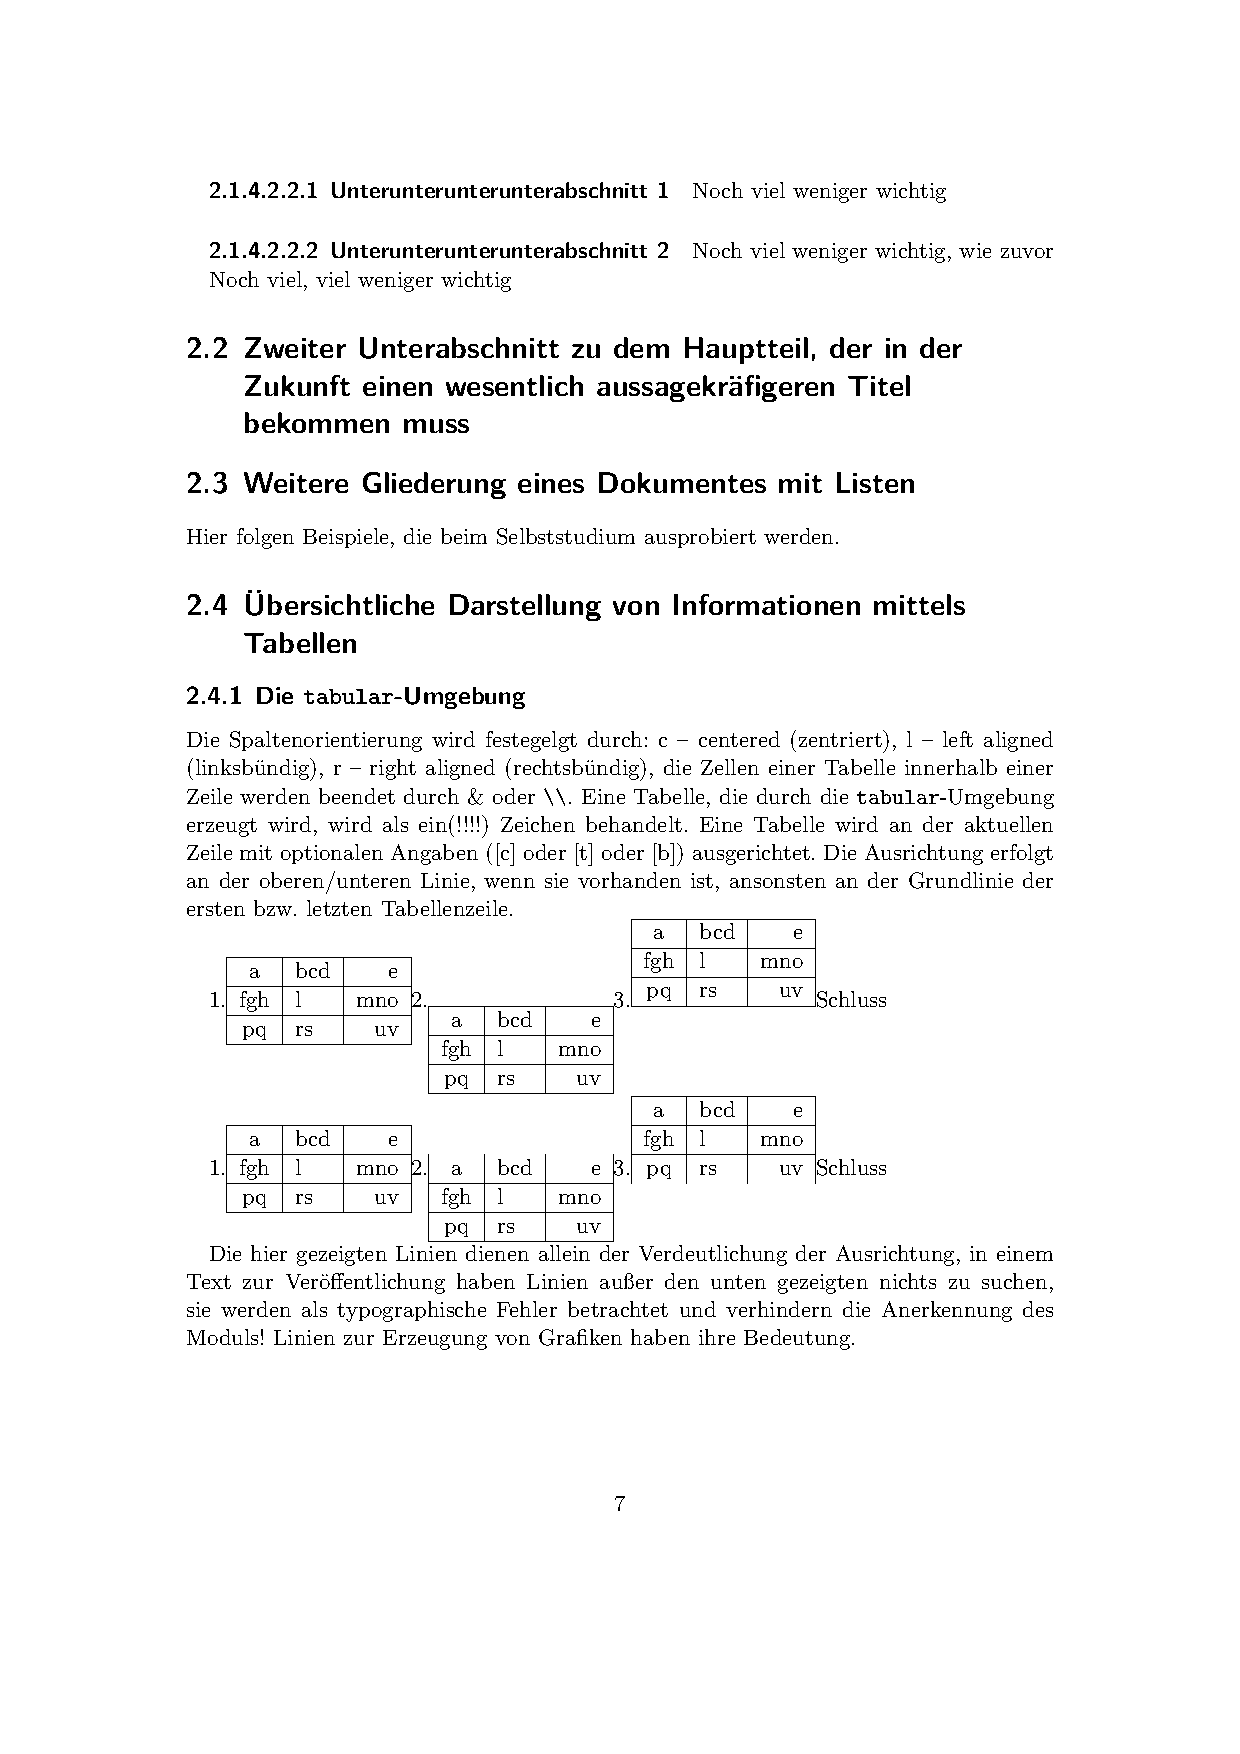
\includegraphics[width=0.7\textwidth]{latex_course_07.pdf} % Erweiterung
                                % muss angegeben werden
    \caption{Ein Ausschnitt aus der vorliegenden Arbeit} % Bilder haben
                                % Unterschriften!
    \label{fig:raster}
\end{figure}


\section{Grafiken und \LaTeX}
\label{sec:grafiken-und-latex}

Es gibt etliche Pakete, mit denen (Linien-)Grafiken mit \LaTeX-Befehlen erzeugt
werden können:
\begin{enumerate}
  \item \texttt{pict2e} als Erweiterung der \LaTeX-immanenten
    \texttt{picture}-Umgebung,
  \item \texttt{pstricks}, das entsprechend der Dokumentation
    \textit{PostScript macros for Generic \TeX} bereitstellt, und
  \item \texttt{tikz}, was für \textit{TikZ is kein Zeichenprogramm} steht,
    und eine große Sammlung von Bibliotheken bereitstellt, die auf PGF
    basieren. Die Originaldokumentation sagt dzu aus: "`\textit{PGF is a
      TeX macro package for generating graphics. It is platform- and
      format-independent and works together with the most important TeX
      backend drivers, including pdftex and dvips. It comes with a
      user-friendly syntax layer called TikZ.}"'
  \item \ldots{}
\end{enumerate}
Beispiele zu den erstgenannten Paketen finden sich in, hier werden nur
\texttt{tikz} und ein paar Erweiterungen vorgestellt.

\subsection{\texttt{tikz} als universelles Makropaket zum Programmieren von
  Grafiken}
\label{sec:als-univ-makr}

\texttt{tikz} stellt zwei Möglichkeiten der Erzeugung von Grafiken bereit:
\begin{enumerate}
  \item Den Befehl \cs{tikz}, der \texttt{tikz}-Makros als Argument(e)
    benötigt, und der \textit{inline}-Grafiken wie
    \tikz \draw (0, 0) -- (1mm, 1mm); erzeugt, eine fehlende Einheit wird
    als cm interpretiert.
  \item Die Umgebung \texttt{tikzpicture}, die eigenständige Grafiken aus
    \texttt{tikz}-Makros erzeugt.
\end{enumerate}
\textbf{Hinweis:} Jedes Makro muss mit einem Semikolon abgeschlossen werden.


\subsubsection{Elementare Beispiele}
\label{sec:elementare-beispiele}

Um die Beispiele besser verstehen zu können, wird zu einem Trick gegriffen:
\begin{enumerate}
  \item mit der Umgebung \texttt{verbatimwrite} aus dem Paket \texttt{moreverb}
    werden Kommandos in eine Datei geschrieben.
  \item mit dem Kommando \lstinline|\lstinputlisting| wird diese Datei
    eingelesen und wörtlich wiedergegeben.
  \item mit dem Kommando \lstinline|\input| wird diese Datei
    eingelesen und formatiert.
\end{enumerate}

\begin{enumerate}
  \item Ein Linienzug wird erzeugt mit
\begin{verbatimwrite}{../../../shared/figures/linienzug.tex}
\tikz \draw[thick,rounded corners=2pt] % eine "dicke" Linie, Ecken werden
                                       % abgerundet
(0,0) -- (0,2) -- (1,3.25) -- (2,2) -- % -- verbindet zwei Punkte durch
(2,0) -- (0,2) -- (2,2) -- (0,0) -- (2,0);  % eine Gerade
\end{verbatimwrite}
    \lstinputlisting{../../../shared/figures/linienzug.tex}

    \tikz \draw[thick,rounded corners=2pt] % eine "dicke" Linie, Ecken werden
                                       % abgerundet
(0,0) -- (0,2) -- (1,3.25) -- (2,2) -- % -- verbindet zwei Punkte durch
(2,0) -- (0,2) -- (2,2) -- (0,0) -- (2,0);  % eine Gerade

  \item Ein Linienzug mit Ecken wird erzeugt mit
\begin{verbatimwrite}{../../../shared/figures/linienzug_eck.tex}
  \tikz \draw[thick]                   % eine "dicke" Linie
  (0,0) -| (2,2) |- (4, 4);            % Punkte werden über Eck
                                       % verbunden
\end{verbatimwrite}
    \lstinputlisting{../../../shared/figures/linienzug_eck.tex}

      \tikz \draw[thick]                   % eine "dicke" Linie
  (0,0) -| (2,2) |- (4, 4);            % Punkte werden über Eck
                                       % verbunden

  \item Eine Kurve wird erzeugt mit
\begin{verbatimwrite}{../../../shared/figures/kurve.tex}
\begin{tikzpicture}
    \filldraw [gray] (0,0) circle [radius=2pt]
    (1,1) circle [radius=2pt]
    (2,2) circle [radius=2pt]
    (2,0) circle [radius=2pt];
    \draw (0,0) .. controls (1,1) and (2,2) .. (2,0);
\end{tikzpicture}
\end{verbatimwrite}
    \lstinputlisting{../../../shared/figures/kurve.tex}

    \begin{tikzpicture}
    \filldraw [gray] (0,0) circle [radius=2pt]
    (1,1) circle [radius=2pt]
    (2,2) circle [radius=2pt]
    (2,0) circle [radius=2pt];
    \draw (0,0) .. controls (1,1) and (2,2) .. (2,0);
\end{tikzpicture}

  \item (Wiederholte) Kreise in einem verschiedenfarbig gezeichneten Gitter anordnen:
\begin{verbatimwrite}{../../../shared/figures/kreise_wdh.tex}
\tikz {%
  % Gitter zur besseren Einordnung der Kreise
  \draw[step=.5cm, blue] (-0.6,-0.6) grid (9.6,0.6);
  \draw[step=.5cm, help lines, red, xshift=0.25cm, ystep=0cm] (-0.6,-0.6) grid (9.3,0.6);
  \draw[step=.5cm, help lines, green, yshift=0.25cm, xstep=0cm] (-0.6,-0.6) grid (9.6,0.3);

  \foreach \x in {0,...,9}
    \draw (\x,0) circle (0.4cm);       % Mittelpunkt und Radius eines Kreises
}
\end{verbatimwrite}
    \lstinputlisting{../../../shared/figures/kreise_wdh.tex}

    \tikz {%
  % Gitter zur besseren Einordnung der Kreise
  \draw[step=.5cm, blue] (-0.6,-0.6) grid (9.6,0.6);
  \draw[step=.5cm, help lines, red, xshift=0.25cm, ystep=0cm] (-0.6,-0.6) grid (9.3,0.6);
  \draw[step=.5cm, help lines, green, yshift=0.25cm, xstep=0cm] (-0.6,-0.6) grid (9.6,0.3);

  \foreach \x in {0,...,9}
    \draw (\x,0) circle (0.4cm);       % Mittelpunkt und Radius eines Kreises
}

  \item Koordinaten an Punkten notieren:
\begin{verbatimwrite}{../../../shared/figures/punkte.tex}
\begin{tikzpicture}
    \draw (0,0) circle [radius=2pt] node [anchor=east]{(0, 0)};
    \draw (1,1) circle [radius=2pt] node [anchor=north]{(1, 1)};
    \fill (2,2) circle [radius=2pt] node [anchor=south]{(2, 2)};
    \draw[thick] (3,1) circle [radius=2pt] node [anchor=north west]{(3, 1)};
    \draw[red, fill=green] (4,0) circle [radius=2pt]
        node [anchor=west, black]{(4, 0)};
\end{tikzpicture}
\end{verbatimwrite}
    \lstinputlisting{../../../shared/figures/punkte.tex}

    \begin{tikzpicture}
    \draw (0,0) circle [radius=2pt] node [anchor=east]{(0, 0)};
    \draw (1,1) circle [radius=2pt] node [anchor=north]{(1, 1)};
    \fill (2,2) circle [radius=2pt] node [anchor=south]{(2, 2)};
    \draw[thick] (3,1) circle [radius=2pt] node [anchor=north west]{(3, 1)};
    \draw[red, fill=green] (4,0) circle [radius=2pt]
        node [anchor=west, black]{(4, 0)};
\end{tikzpicture}

  \item Grafische Elemente an bestimmten Stellen positionieren:
\begin{verbatimwrite}{../../../shared/figures/node_pos.tex}
\begin{tikzpicture}
    \begin{scope}[name prefix = top-]
        \node (A) at (0,1) {A};
        \node (B) at (1,1) {B};
        \draw (A) -- (B);
    \end{scope}
    \begin{scope}[name prefix = bottom-]
        \node (A) at (0,0) {A};
        \node (B) at (1,0) {B};
        \draw (A) -- (B);
    \end{scope}

    \draw [red] (top-A) -- (bottom-B);
\end{tikzpicture}
\end{verbatimwrite}
    \lstinputlisting{../../../shared/figures/node_pos.tex}

    \begin{tikzpicture}
    \begin{scope}[name prefix = top-]
        \node (A) at (0,1) {A};
        \node (B) at (1,1) {B};
        \draw (A) -- (B);
    \end{scope}
    \begin{scope}[name prefix = bottom-]
        \node (A) at (0,0) {A};
        \node (B) at (1,0) {B};
        \draw (A) -- (B);
    \end{scope}

    \draw [red] (top-A) -- (bottom-B);
\end{tikzpicture}


  \item Bäume mit der Bibliothek \texttt{trees} (in \texttt {twp-cfg.tex}
    muss die Zeile
\begin{lstlisting}
\usetikzlibrary{trees}          % Produzieren von Baumstrukturen
\end{lstlisting}
    stehen) konstruieren:
\begin{verbatimwrite}{../../../shared/figures/path_tree.tex}
% Voreinstellungen für Elemente des Baumes
\tikzset{directory/.style={rectangle, rounded corners, draw,
        font=\ttfamily, fill=blue!20}}
\tikzset{file/.style={rectangle, draw, font=\ttfamily, fill=green!10}}

\begin{tikzpicture}[level distance=7.5mm]%
    \node[directory] {\ldots} %
        [edge from parent fork down]%
    child[sibling distance=30mm] {node[directory] {a}} %
    child {node[directory] {b-directory} %
      child {node[directory] {c} %
        child{node[file] {MyClass.java}}} %
    }
    child[sibling distance=30mm] {node[file] {README.md}};
\end{tikzpicture}
\end{verbatimwrite}
    \lstinputlisting{../../../shared/figures/path_tree.tex}

    % Voreinstellungen für Elemente des Baumes
\tikzset{directory/.style={rectangle, rounded corners, draw,
        font=\ttfamily, fill=blue!20}}
\tikzset{file/.style={rectangle, draw, font=\ttfamily, fill=green!10}}

\begin{tikzpicture}[level distance=7.5mm]%
    \node[directory] {\ldots} %
        [edge from parent fork down]%
    child[sibling distance=30mm] {node[directory] {a}} %
    child {node[directory] {b-directory} %
      child {node[directory] {c} %
        child{node[file] {MyClass.java}}} %
    }
    child[sibling distance=30mm] {node[file] {README.md}};
\end{tikzpicture}

\end{enumerate}


\subsubsection{Das Bezeichnen vorgegebener Abbildungen}
\label{sec:das-beze-vorg}

Es gibt häufig den Fall, dass ein gegebenes Bild mit zusätzlichen
Bezeichnungen versehen werden muss.

Zunächst werden die in einem ungleichmäßig skalierten Bildschirmfoto die
Linien eingezeichnet, die beim \texttt{trim} eingesetzt wurden.

\begin{tikzpicture}
    \tikzset{every ellipse node/.style={draw,
        color=red, text=black, line width=2pt}}
    \pgftext[bottom, left, x=0pt, y=0pt]{% Ausrichtung des Bildes
                                % erfolgt an seiner linken Unterkante,
                                % es wird nicht in x- oder y-Richtung
                                % verschoben
      \includegraphics[width=15cm, height=10cm]{bildschirmfoto}}; % das Bild auf
                                % eine feste Breite skaliert
    \draw[help lines, white, thick] (0, 0) grid (15,10);%
    \draw[red, very thick] (7.5, 0) -- (7.5, 10)
                           (7.5, 5) -- (15, 5)
                           (11.25, 5) -- (11.25, 10)
                           (7.5, 7.5) -- (11.25, 7.5);%
    \node[white] at (9.375, 6.25){trimmed};%
\end{tikzpicture}

Dann wird in einem gleichmäßig skalierten Bildschirmfoto der Kopf des
Nachrichtensprechers markiert.

\begin{tikzpicture}
    \tikzset{every ellipse node/.style={draw,
        color=red, text=black, line width=2pt}}
    \pgftext[bottom, left, x=0pt, y=0pt]{%
      \includegraphics[width=16cm]{bildschirmfoto}}; % das Bild auf
                                % eine feste Breite skaliert
      % \draw[help lines, white, thick] (0, 0) grid (16, 9);%
      \draw[white, very thick] (11.75, 7) ellipse [x radius=0.75cm, y radius=1.5cm];
\end{tikzpicture}


\subsection{\texttt{pgfplots} als Paket zur Darstellung von Funktionen}

Eine häufig auftretende Aufgabenstellung ist die Darstellung beliebiger
Funktionen. Prinzipiell kann das mit den nun bekannten Mitteln von
\texttt{tikz} erledigt werden, besser geeignet ist das Paket \texttt{pgfplots}.
Zusätzlich zum Laden des Paketes sollte in \texttt{twp-cfg.tex} die
Kompatibilitätsstufe vermerkt werden.

\begin{enumerate}
  \item Eine Funktion \(f: \mathcal R \rightarrow \mathcal R\):
\begin{verbatimwrite}{../../../shared/figures/r_to_r_gnuplt.tex}
\begin{tikzpicture}
    \begin{axis}            % das Koordinatensystem wird mit
                            % der Umgebung axis erzeugt
        \addplot[           % ein Plot wird hinzugefügt
          id=parable,
          domain=-5:5,      % der Definitionsbereich
        ] gnuplot {4*x**2 - 5}% die Funktion, setzt das Programm
        % gnuplot voraus
        node [pin=180:{$4x^2-5$}]{}; % Legende der Grafik
    \end{axis}
\end{tikzpicture}
\end{verbatimwrite}
    \lstinputlisting{../../../shared/figures/r_to_r_gnuplt.tex}

    \begin{tikzpicture}
    \begin{axis}            % das Koordinatensystem wird mit
                            % der Umgebung axis erzeugt
        \addplot[           % ein Plot wird hinzugefügt
          id=parable,
          domain=-5:5,      % der Definitionsbereich
        ] gnuplot {4*x**2 - 5}% die Funktion, setzt das Programm
        % gnuplot voraus
        node [pin=180:{$4x^2-5$}]{}; % Legende der Grafik
    \end{axis}
\end{tikzpicture}


  \item Dieselbe Funktion \(f: \mathcal R \rightarrow \mathcal R\) mit
    \TeX{} als Datenprozessor, zu beachten ist die andere Darstellung der
    Potenz -- gnuplot: \lstinline|4*x**2 - 5|, also zwei Sternchen, \TeX:
    \lstinline|4*x^2-5|.
\begin{verbatimwrite}{../../../shared/figures/r_to_r_tex.tex}
  \begin{tikzpicture}
      \begin{axis}            % das Koordinatensystem wird mit
                              % der Umgebung axis erzeugt
          \addplot[             % ein Plot wird hinzugefügt
            domain=-5:5         % der Definitionsbereich
          ] { 4*x^2-5 }         % die Funktion
          node [pin=180:{$4x^2-5$}]{}; % Legende der Grafik
      \end{axis}
  \end{tikzpicture}
\end{verbatimwrite}
    \lstinputlisting{../../../shared/figures/r_to_r_tex.tex}

      \begin{tikzpicture}
      \begin{axis}            % das Koordinatensystem wird mit
                              % der Umgebung axis erzeugt
          \addplot[             % ein Plot wird hinzugefügt
            domain=-5:5         % der Definitionsbereich
          ] { 4*x^2-5 }         % die Funktion
          node [pin=180:{$4x^2-5$}]{}; % Legende der Grafik
      \end{axis}
  \end{tikzpicture}


  \item Noch einmal dieselbe Funktion
    \(f: \mathcal R \rightarrow \mathcal R\) mit \TeX{} als Datenprozessor,
    jetzt mit einer zusätzlichen Achsenbeschriftung und einem Vergleich mit
    Messpunkten.
\begin{verbatimwrite}{../../../shared/figures/r_to_r_vgl.tex}
  \begin{tikzpicture}
      \begin{axis}[           % das Koordinatensystem wird mit
                              % der Umgebung axis erzeugt,
                              % hier zusätzliche Optionen
            xlabel=\(x\),
            ylabel={\(y=f(x)=4x^2 - 5\)} % {...} wegen der
                              % Leerzeichen
          ]
          \addplot[           % ein Plot wird hinzugefügt
            domain=-5:5,      % der Definitionsbereich
            color=blue,
            mark=x            % berechnete Punkte werden mit
                              % einem x markiert
          ] { 4*x^2-5 }       % die Funktion
          node [pin=180:{$4x^2-5$}]{}; % Legende der Grafik
          \addplot[
            domain=-5:5,
            color=green,
            mark=*
          ]
          coordinates {
            (-4, 59)
            (0, -5)
            (1, -1)
            (2, 9)
            (5, 95)
          };
      \end{axis}
  \end{tikzpicture}
\end{verbatimwrite}
    \lstinputlisting{../../../shared/figures/r_to_r_vgl.tex}

      \begin{tikzpicture}
      \begin{axis}[           % das Koordinatensystem wird mit
                              % der Umgebung axis erzeugt,
                              % hier zusätzliche Optionen
            xlabel=\(x\),
            ylabel={\(y=f(x)=4x^2 - 5\)} % {...} wegen der
                              % Leerzeichen
          ]
          \addplot[           % ein Plot wird hinzugefügt
            domain=-5:5,      % der Definitionsbereich
            color=blue,
            mark=x            % berechnete Punkte werden mit
                              % einem x markiert
          ] { 4*x^2-5 }       % die Funktion
          node [pin=180:{$4x^2-5$}]{}; % Legende der Grafik
          \addplot[
            domain=-5:5,
            color=green,
            mark=*
          ]
          coordinates {
            (-4, 59)
            (0, -5)
            (1, -1)
            (2, 9)
            (5, 95)
          };
      \end{axis}
  \end{tikzpicture}

\end{enumerate}


\section{Mathematischer Formelsatz}

Zwei Varianten: \TeX-spezifisch und \LaTeX-spezifisch, letztere ist unbedingt
vorzuziehen!

\begin{tabular}{llll}
  \toprule
  & \TeX & \LaTeX{} lang & \LaTeX{} kurz\\
  \midrule
  \textit{inline} & \lstinline|$ ... $| & \lstinline|\begin{math} ... \end{math}| & \lstinline|\( ... \)| \\
  \textit{display} & \lstinline|$$ ... $$| & \lstinline|\begin{displaymath} ... \end{displaymath}|& \lstinline|\[ ... \]| \\
  \bottomrule
\end{tabular}

\textit{inline} bedeutet: \(3+4=7\), dahingegen wird \textit{display} so
formatiert: \[3+4=7\]. Es gibt viele Automatiken in \TeX: Zahlen werden
automatisch als \textit{inline math} erkannt, es wird automatisch
unterschieden zwischen Bindestrich und Minuszeichen, ebenso wird Vorzeichen
von Operator unterschieden:
\[\mbox{3-4, aber } 3-4=-1\]

Der Mathematikmodus stellt viele zusätzliche Befehle bereit, so wird der
Unterstrich benutzt, um Indizes zu kennzeichnen: \(a_{ij}\).\footnote{Die
  Klammern sind wichtig: \(a_{ij} \ne a_ij\).} Entsprechend wird das Dach
für Exponenten benutzt: \(x^{2}\). Text wird im mathematischen Formelsatz
kursiv gesetzt, Funktionen hingegen aufrecht: \(f(x) = \sin x\). Es gibt
die üblichen mathematischen Funktionen in der Schreibweise
\cs{}\meta{Funktionsname}, also etwa \(\cos \pi = -1\).


\subsection{Skalare Größen/Gleichungen}

Wichtige mathematische Bezeichnungen sind
\(\sum_{i=1}^{n}i=\frac{n\cdot(n+1)}{2}\) oder auch
\[\sum_{i=1}^{n}i=\frac{n\cdot(n+1)}{2}\]

Der \textit{displaymath}-Modus sorgt für größere Zeichen und bessere
Übersicht!

\[\int\limits_{-1}^{1} x dx = 0\]

Für Wurzeln gibt es \lstinline|\sqrt[root]{arg}|: \(\sqrt[3]{27}=3\)

Es ist eine typografische Unart, die Menge der reellen Zahlen mit
\(\mathbb{R}\) zu beschreiben, richtig ist \(\mathcal{R}\).

Grenzwerte werden so geschrieben:
\( \lim\limits_{x\rightarrow0}\frac{\sin x}{x}=0 \mbox{ oder }
\lim_{x\rightarrow0}\frac{\sin x}{x}=0 \) aber
\[
    \lim\limits_{x\rightarrow0}\frac{\sin x}{x}=0 \mbox{ oder }
    \lim_{x\rightarrow0}\frac{\sin x}{x}=0
\]

Im Mathematikmodus gibt es keinen Umbruch!!! Wenn mehrere Zeilen gebraucht
werden, muss man mit geeigneten Umgebungen wie \texttt{eqnarray} arbeiten:
\begin{eqnarray}
  \label{eq:sin}%
  \sin x & = & \sum_{i=0}^{\infty}(-1)^{i}\frac{x^{2i+1}}{(2i+1)!}
  \\
  \label{eq:sin_expl}       & = & x - \frac{1}{3!}x^{3} + \frac{1}{5!}x^{5} - \ldots + \ldots
\end{eqnarray}
\textbf{Hinweise:}
\begin{enumerate}
  \item \texttt{eqnarray} ist eine spezielle Tabelle, es besteht aus drei
    Spalten, das Gleichheitszeichen muss zwischen zwei kaufmännische Unds
    gesetzt werden.
  \item Jede Zeile bekommt automatisch eine Nummer, auf die man sich
    beziehen kann, etwa so: Die Taylorentwicklung der \(\sin\)-Funktion
    wird in Gleichung \ref{eq:sin} gezeigt, Gleichung \ref{eq:sin_expl}
    zeigt die ausgeführte Summenbildung.

    \lstinline|\cref| funktioniert gemäß ...  mit der
    \texttt{eqnarray}-Umgebung nicht, es liefert hier \cref{eq:sin}(?)! Es
    wird empfohlen, die analogen Umgebungen des \texttt{amsmath}-Paketes zu
    benutzen.
  \item \texttt{eqnarray*} liefert keine Nummern.
  \item Eine Nummer kann zeilenweise unterdrückt werden mit dem
    Befehl \lstinline|\nonumber|.
\end{enumerate}

Eine einfachere Beschreibung von mathematischen Zusammenhängen ist mit dem
Paket \texttt{amsmath} möglich, dann funktioniert
auch \lstinline|\cref|. Das obige Beispiel lässt sich dann so schreiben:
\begin{equation}
    \begin{split}
      \label{eq:sin_ams}%
      \sin x &=  \sum_{i=0}^{\infty}(-1)^{i}\frac{x^{2i+1}}{(2i+1)!}
      \\
             &=  x - \frac{1}{3!}x^{3} + \frac{1}{5!}x^{5} - \ldots + \ldots
    \end{split}
\end{equation}
\cref{eq:sin_ams} zeigt die Taylorentwicklung der \(\sin\)-Funktion.

Analog zu \texttt{eqnarray} gibt es  \texttt{align}
\begin{align}
  \label{eq:ams_sin}%
  \sin x &=  \sum_{i=0}^{\infty}(-1)^{i}\frac{x^{2i+1}}{(2i+1)!}
  \\
  \label{eq:ams_sin_expl}        &=  x - \frac{1}{3!}x^{3} + \frac{1}{5!}x^{5} - \ldots + \ldots
\end{align}
Zur Darstellung von Fallunterscheidungen gibt es \texttt{cases}:
\begin{equation}
    \label{eq:fakultaet_00}
    n! =
    \begin{cases}
      1 & n=1\\
      n(n-1)! & n > 1
    \end{cases}
\end{equation}
\cref{eq:fakultaet_00} kommt ohne Text aus, besser ist es mit einer Erklärung,
wie es in \cref{eq:fakultaet_01} gezeigt wird:
\begin{equation}
    \label{eq:fakultaet_01}
    n! =
    \begin{cases}
      1 & \text{für } n=1\\          % lokale Umschltung in den
      n(n-1)! & \text{für den Fall } n > 1    % Textmodus
    \end{cases}
\end{equation}


\subsection{Vektorielle Größen/Gleichungen}

Ein Vektor im \(n\)-dimensionalen Raum wird beschrieben durch
\(\vec{x} \in \mathcal{R}^{n}\). Komponentenweise wird er beschrieben durch
\(\vec{x} = \left(              % \left leitet eine bel. Klammer
    % in der passenden Größe eine
    \begin{array}{c}
      x_{1} \\ \vdots \\ x_{n}  % es gibt neben \vdots (vertical)
      % auch \ldots (lower)
      % \cdots (central)
      % \ddots (diagonal)
      % als Befehle zum Beschreiben einer
      % Folge von Punkten
    \end{array}
\right)                   % \right ist verpflichtend nach einem $\left$
\)

Damit lässt sich ein Gleichungssystem schreiben als
\[
    \underbrace{
      \left(
          \begin{array}{*{4}{c}}
            a_{11} & a_{12} & \cdots & a_{1n} \\
            a_{21} & a_{22} & \cdots & a_{2n} \\
            \vdots & \vdots & \ddots & \vdots \\
            a_{m1} & a_{m2} & \cdots & a_{mn} \\
          \end{array}
      \right)
      \cdot
      \left(
          \begin{array}{c}
            x_{1} \\
            x_{2} \\
            \vdots \\
            x_{n}
          \end{array}
      \right)
    }_{\text{linke Seite}}
    =
    \underbrace{
      \left(
          \begin{array}{c}
            b_{1} \\
            b_{2} \\
            \vdots \\
            b_{n}
          \end{array}
      \right)
    }_{\text{rechte Seite}}
\]
kurz:
\[
    A\cdot\vec{x}=\vec{b}
\]
oder mit Nummerierung der Formel
\begin{equation}
    A\cdot\vec{x}=\vec{b}
\end{equation}


\section{Feinheiten des Drucksatzes mit \TeX/\LaTeX}

\subsection{Gestaltung einer Titelseite}

Bessere Gestaltung einer Titelseite erfolgt durch
\begin{itemize}
  \item besondere Schrifttypen (Fonts) in unterschiedlichen Größen,
  \item grafische Elemente (Linien in unterschiedlichene Dicken und
    Richtungen) und
  \item evtl. Logos.
\end{itemize}

Es wird unterschieden zwischen Brotschrift, wie sie für den laufenden Text
gebraucht wird, und Auszeichungsschrift, die für Überschriften eingesetzt
wird.

Als Brotschrift wird der besseren Lesbarkeit halber eine Serifen-behaftete
Schrift ausgewählt (Standard in \texttt{scr}-Paketen: eine von der Times
abgeleitete Schrift -- auch als Antiqua bezeichnet, da mit einer solchen
Schrift römische Tempel beschrieben worden sind, daher auch der Name
\textit{modern roman} -- , definiert durch die Serifen eine Grundlinie, die
die Augen der Schrift besser folgen lässt).

Als Auszeichungsschrift wird eine Schrift ausgewählt, die viele
Eigenschaften mit der Brotschrift gemeinsam hat, die sich aber dennoch
deutlich unterscheidet (Standard in \texttt{scr}-Paketen: eine serifenlose,
fette Schrift -- als Helvetica bezeichnet).

Diese Schriften werden unterschiedlichen Größen eingesetzt: von {\tiny ganz
  winzig} bis zu {\Huge riesig groß}. \lstinline|\tiny|
und \lstinline|\Huge| sind Schrift\emph{attribute}, die ab sofort bis zum
Gruppenende gelten.

\textnormal{Das ist Brotschrift} und \textsf{das ist Auszeichungsschrift},
\textnormal{das ist normale Brotschrift} und \textsf{\bfseries das ist
  fette Auszeichungsschrift}.

Merkregel: Innerhalb eines laufenden Textes wird \emph{niemals}%
\footnote{typografischer Fehler, \ldots} fett gedruckt, wenn etwas
\emph{hervorgehoben} werden soll, dann durch Betonung
(\textit{emphasize}, \lstinline|\emph|).

Linien können gezeichnet werden
\begin{itemize}
  \item horizontal: \rule{220pt}{2pt}
  \item vertikal: \rule{1pt}{22pt}
\end{itemize}
Die Größenangaben werden typischerweise in pt gemacht. Die Einzelheiten dazu
finden sich im Kommertar zu \texttt{titel.tex}.


\subsection{Nicht-horizontale Textausrichtung}

Der Standard im Drucksatz ist die horizontale Textausrichtung des Fließtextes.
Es gibt aber Situationen, in denen eine andere Ausrichtung sinnvoll oder sogar
erforderlich ist. Dafür gibt es das Paket \texttt{rotating.sty}.

\subsubsection{Gedrehte Tabellen}

Sehr breite Tabellen passen nicht in den Satzspiegel, vgl.
\cref{tab:marokko-brasilien}.
\begin{table}[htb]
    \centering%
    \caption{Statistik des Spiels Marokko - Brasilien}
    \label{tab:marokko-brasilien}
    \begin{tabular}{*{6}{p{2.5cm}}}
      \toprule%
      eigene Tore & gegnerische Tore & gelbe Karten & rote Karten &
                                                                    Abseitstellungen & Ballbesitz \\\midrule
      1 & 0 & 2 & 0 & 5 & 30 \% \\\bottomrule
    \end{tabular}
\end{table}

Die Abhilfe ist die gedrehte Tabelle, vgl.
\cref{tab:marokko-brasilien-sideways}.
\begin{sidewaystable}[p]
    \centering%
    \caption{Statistik des Spiels Marokko - Brasilien}
    \label{tab:marokko-brasilien-sideways}
    \begin{tabular}{*{6}{p{2.5cm}}}
      \toprule%
      eigene Tore & gegnerische Tore & gelbe Karten & rote Karten &
                                                                    Abseitstellungen & Ballbesitz \\\midrule
      1 & 0 & 2 & 0 & 5 & 30 \% \\\bottomrule
    \end{tabular}
\end{sidewaystable}

Die Breite einer Tabelle hängt häufig von den Spaltenüberschriften ab,
wie in den Beispeilen \cref{tab:marokko-brasilien} und
\cref{tab:marokko-brasilien-sideways} gut zu sehen ist.

Eine Spaltenüberschrift kann schmaler werden, wenn sie gedreht wird,
vgl. \cref{tab:marokko-brasilien-narrow}.
\begin{table}[htb]
    \centering%
    \caption{Statistik des Spiels Marokko - Brasilien}
    \label{tab:marokko-brasilien-narrow}
    \begin{tabular}{*{6}{l}}
      \toprule%
      \begin{sideways}    % dreht den Inhalt um 90° gegen den Uhrzeigersinn
          eigene Tore
      \end{sideways} & \begin{rotate}{60} % dreht den Inhalt um 60° gegen
          % den Uhrzeigersinn, fordert keinen eigenen Platz
          % ein, \toprule wird falsch gesetzt
          % ein \settoheight{\gnat}{text} würde hier
          % helfen (vgl. \settowidth{\gnat}{text})
          gegnerische Tore
      \end{rotate} & \begin{turn}{30} % dreht den Inhalt um 30° gegen
          % den Uhrzeigersinn, fordert eigenen Platz
          % ein, \toprule wird richtig gesetzt
          gelbe Karten
      \end{turn} & rote Karten &
                                 Abseitstellungen & Ballbesitz \\\midrule
      1 & 0 & 2 & 0 & 5 & 30 \% \\\bottomrule
    \end{tabular}
\end{table}


\section{Verschiedenes}

Hier werden die Themen behandelt, die
\begin{itemize}
  \item nützlich (eigene Definitionen zur Abkürzung häufig benutzter
    Begriffe, ein Seitenlayout mit Zeitangabe) oder
  \item unverzichtbar (Erstellen einer Bibliographie/eines
    Literaturverzeichnisses)
\end{itemize}
für das Erstellen einer Abschlussarbeit sind.

\subsection{Eigene Definitionen}%
\label{sec:eigene-definitionen}

In \TeX{} ist es möglich, mit dem Makro \lstinline|\def| eigene Makros
zu definieren. Diese werden expandiert, d.\,h. durch ihren Inhalt
ersetzt, bis nur noch Primitive auftreten, die dann in Text umgesetzt
werden. Ein einfaches Beispiel:
\begin{verbatimwrite}{../../../shared/texts/def_00.tex}
  \def\dreiA{AAA}
\end{verbatimwrite}
Mit
\lstinputlisting{../../../shared/texts/def_00.tex}
wird ein Makro definiert, das seinen Inhalt direkt ausgibt:
  \def\dreiA{AAA}
\dreiA.

\dreiA\hspace{\fill}\dreiA\hspace{\fill}\dreiA

Die Programmierung von \TeX{} ist damit relativ kompliziert und nur
den \TeX nicians zuzumuten.

\subsection{Programmieren mit \LaTeX}

Die Programmierung mit \LaTeX{} ist wesentlich einfacher gestaltet, es gibt
aber für \LaTeXe{} und \LaTeX3 unterschiedliche Schnittstellen. Da \LaTeX3 jetzt
schon überall unter der Haube arbeitet, wird nur diese Schnittstelle
vorgestellt.

\subsubsection{Eigene Funktionen}

Mit \LaTeX3 ist der Begriff Makro und Makroexpansion aus der Sprachbeschreibung
herausgefallen. Es wird zwar in der Syntaxbeschreibung noch von Expandierung
gesprochen, es geht nun aber immer um Funktionen, Variablen und Strukturen.

An dieser Stelle wird nicht in die Interna eingestiegen, sondern es wird
nur die neue Syntax vorgestellt.


\paragraph{Parameterlose Funktionen}

Zur Definition eigener Kommandos gibt es die Funktion
\begin{lstlisting}[escapechar=@]
\NewDocumentCommand@\marg{cmd}\marg{xargs}\marg{def}@
\end{lstlisting}
\meta{cmd} ist der Name der zu definierenden Funktion, der \cs{} muss
aufgeführt werden, \meta{xargs}
beschreibt die Parameter, \meta{def} ist die Definition der Funktion.

Das Beispiel aus \cref{sec:eigene-definitionen} sieht dann so aus:
\begin{verbatimwrite}{../../../shared/texts/def_01.tex}
\NewDocumentCommand{\iiiA}        % Funktionen dürfen nicht doppelt
                                  % auftreten
                   {}             % es gibt keine Parameter
                   {AAA}          % es sollen drei As gesetzt werden
\end{verbatimwrite}
\lstinputlisting{../../../shared/texts/def_01.tex}

Der Einsatz ist wie oben: \NewDocumentCommand{\iiiA}        % Funktionen dürfen nicht doppelt
                                  % auftreten
                   {}             % es gibt keine Parameter
                   {AAA}          % es sollen drei As gesetzt werden
\iiiA.

Nun etwas sinnvolleres, die Definition einer Abkürzung:
\begin{verbatimwrite}{../../../shared/texts/def_02.tex}
\NewDocumentCommand{\JHf}       % Funktionen dürfen nicht doppelt
                                % auftreten
                   {}           % es gibt keine Parameter
                   {Jobst Hoffmann}  % es soll der Name gesetzt
                                % werden
\end{verbatimwrite}
\lstinputlisting{../../../shared/texts/def_02.tex}

\NewDocumentCommand{\JHf}       % Funktionen dürfen nicht doppelt
                                % auftreten
                   {}           % es gibt keine Parameter
                   {Jobst Hoffmann}  % es soll der Name gesetzt
                                % werden

Zunächst muss die Definition wieder eingelesen werden, bevor sie
benutzt werden kann: \JHf schrieb diesen Text. Es ist zu beachten,
dass auch eigene Funktionen sich nach der grundsätzlichen Syntax von
\TeX/\LaTeX{} arbeiten: ein Funktionsaufruf endet mit dem ersten
Nicht-Buchstaben. Um also nach dem Namen ein Leerzeichen zu erhalten,
muss der Funktionsaufruf mit \{\} beendet werden: \JHf{} schrieb
diesen Text.

\paragraph{Funktionen mit Parametern}

\meta{xargs} beschreibt die Parameter, die der Funktion übergeben werden
können. Es wird hier nur der Fall beschrieben, dass als Argument ein
einzelnes Token oder mehrere mit geschweiften Klammern \{\} umgebene Token
auftreten. Weitere Parameterarten sind \cite{latex_project_22:xparse} zu
entnehmen.

\meta{xargs} ist eine Folge von Buchstaben, wir benutzen nur \texttt{m} und 
\texttt{o}, für jeden dieser Buchstaben mit im Ersatztext der Reihe nach
\lstinline|#1|, \lstinline|#2|, $\ldots$, \lstinline|#9| auftreten, es gibt
auf diese Weise maximal 9 Parameter.


\subparagraph{Umgang mit obligatorischen (engl.: \textit{\_m\_andatory}) Parametern}

Um einen Vektor komponentenweise aufzuschreiben, muss man die
Dimension des zugehörigen Raumes angeben:
\begin{verbatimwrite}{../../../shared/texts/def_03.tex}
  \NewDocumentCommand{\vektor}   % Funktionen dürfen nicht doppelt
                                 % auftreten
                     {m}         % es gibt einen verpflichtenden
                                 % Parameter, die Dimension
                     {           % es sollen die Komponenten
                        \ensuremath{(x_{1},  % eines Vektor
                          \ldots, % beschrieben werden
                                 % \ensuremath: unabhängig
                                 % von Mathematik-Modus
                          x_{#1})}
                     }

\end{verbatimwrite}
\lstinputlisting{../../../shared/texts/def_03.tex}

  \NewDocumentCommand{\vektor}   % Funktionen dürfen nicht doppelt
                                 % auftreten
                     {m}         % es gibt einen verpflichtenden
                                 % Parameter, die Dimension
                     {           % es sollen die Komponenten
                        \ensuremath{(x_{1},  % eines Vektor
                          \ldots, % beschrieben werden
                                 % \ensuremath: unabhängig
                                 % von Mathematik-Modus
                          x_{#1})}
                     }



\vektor{3}, \vektor{n}

\subparagraph{Umgang mit optionalen (engl.: \textit{\_o\_ptional}) Parametern}

Was muss getan werden, wenn weitere Vektoren auftreten? Kann mit der Dimension
besser umgegangen werden? Also: standardmäßig wird im \(\mathcal R^{3}\) 
gearbeitet, es kann aber auch eine andere Dimension genannt werden.

\begin{verbatimwrite}{../../../shared/texts/def_04.tex}
  \NewDocumentCommand{\vektorN}  % Funktionen dürfen nicht doppelt
                                 % auftreten
                     {o m}       % es gibt einen optionalen, den 
                                 % Namen, und einen verpflichtenden
                                 % Parameter, die Dimension
                     {           % es sollen die Komponenten
                       \IfNoValueTF{#1}{\def\dimI{3}}{\def\dimI{#1}}
                       \ensuremath{(#2_{1},  % eines Vektor
                       \ldots,   % beschrieben werden
                                 % \ensuremath: unabhängig
                                 % von Mathematik-Modus
                       #2_{\dimI})
                     }
  }
  
\end{verbatimwrite}
\lstinputlisting{../../../shared/texts/def_04.tex}

  \NewDocumentCommand{\vektorN}  % Funktionen dürfen nicht doppelt
                                 % auftreten
                     {o m}       % es gibt einen optionalen, den
                                 % Namen, und einen verpflichtenden
                                 % Parameter, die Dimension
                     {           % es sollen die Komponenten
                       \IfNoValueTF{#1}{\def\dimI{3}}{\def\dimI{#1}}
                       \ensuremath{(#2_{1},  % eines Vektor
                       \ldots,   % beschrieben werden
                                 % \ensuremath: unabhängig
                                 % von Mathematik-Modus
                       #2_{\dimI})
                     }
  }



\vektorN{x}, \vektorN{y}, \vektorN[n]{x}, \vektorN[n]{y}


\subparagraph{Umdefinieren von Umgebungen}

Wenn eine Umgebung nicht so arbeitet, wie der Autor es sich vorstellt, 
kann sie umdefiniert werden.

Ein Vers von Wilhelm Busch:
\begin{verse}
  Eins, zwei, drei im Sauseschritt, \\
  eilt die Zeit, wir eilen mit.
\end{verse}

Der Autor wünscht sich aber
\begin{center}
  Eins, zwei, drei im Sauseschritt, \\
  eilt die Zeit, wir eilen mit.
\end{center}

Die einfachere Lösung ist:
\lstinline|\renewenvironment{envname}[args]{begdef}{enddef}|, also
\renewenvironment{verse}{\begin{center}}{\end{center}}

Damit sieht das so aus:

Ein Vers von Wilhelm Busch:
\begin{verse}
  Eins, zwei, drei im Sauseschritt, \\
  eilt die Zeit, wir eilen mit.
\end{verse}

Dieses Umdefinieren von Umgebungen ermöglicht es, per Programm das Aussehen
eines Dokumentes zu verändern. Dies \emph{muss unbedingt} bei einem
Brief/Anschreiben gemacht werden: Blocksatz in einem solchen Dokument darf
nicht genutzt werden!!!!!

Das Neudefinieren einer Umgebung durch sich selbst funktioniert nicht, daher
\ldots.


\subsection{Seitenlayout -- Festlegen von Kopf- und Fußzeile}

Es gibt eine Standardeinstellung für das Aussehen von  Kopf- und Fußzeile,
die für das praktische Arbeiten aber nicht hilfreich ist.

Zum Koma-Skript-Paket gibt es ein weiteres Paket, mit alle Wünsche erfüllt
werden können. Die erforderlichen Einstellungen werden in der
Konfigurationsdatei \texttt{twp-cfg.tex} vorgenommen.


\subsection{Vervollständigung eines Dokumentes}

\subsubsection{Die Bibliographie bzw. das Literaturverzeichnis}

Das Kennzeichen einer wissenschaflichen Arbeit ist das Belegen von Aussagen
durch
\begin{itemize}
  \item eigene Beweise und
  \item Verweise auf anerkannte(!!!!!) Quellen. Dies sind nicht einfache 
    Angaben wie: der bekannte Forscher X.~Y. hat herausgefunden, sondern
    Verweise auf seriöse Veröffentlichungen wie
    \begin{itemize}
      \item Bücher in bekannten Verlagen, die wissenschaftliche Werke
        veröffentlichen,
      \item Artikel in wissenschaftlichen Zeitschriften, die von anderen
        Wissenschaftlern geprüft worden sind,
      \item (bedingt) Artikel in Zeitschriften, die sich mit Themen aus dem
        jeweiligen Fachgebiet beschäftigen und
      \item Veröffentlichungen im Internet, wenn der Autor über ein 
        geeignetes Renommee verfügt.
    \end{itemize}
    Auch Tagungsbände, Forschungsberichte und ähnliche Publikationen sind 
    solche seriöse Veröffentlichungen.
    
    Man muss aber aufpassen: es werden Gesellschaften gegründet, die einzig
    und allein dem Ziel des Gründers untergeordnet sind, so beispielsweise
    Forschungsinstitute im Auftrag der Zigarettenindustrie, die sich mit
    den mangelnden Beweisen für die Schädlichkeit des Rauchens beschäftigt
    haben. Die Frage nach der Herkunft von Geldern ist immer zu klären!
\end{itemize}

Wie geht man vor?
\begin{enumerate}
  \item Man wählt einen passenden Namen für die Bibiliographie-Datenbank,
    muss mit .bib enden.
  \item Man fügt einen \lstinline|\addbibresource{bibliographic resource}|
    Eintrag unter der Paket auswahl \texttt{biblatex ein}, der Eintrag
    darf eine Pfadangabe beinhalten.
  \item Man macht einen Eintrag in der .bib-Datenbank (Bibliographie
    \(rightarrow\) passender Eintrag), Alt...-Einträge müssen passend 
    gelöscht werden.
  \item Die Bibliographie muss aufgeräumt werden
  \item Nach \lstinline|\backmatter| muss der Befehl
    \lstinline|\printbibliography| mit eventuellen Optionen aufgeführt
    werden.
  \item Fertig!
\end{enumerate}


\subsubsection{Stichwortverzeichnis -- Index}

Das Erstellen eines Stichwortverzeichnisses ist beim Schreiben einer
Bachelorarbeit nicht erforderlich.


\subsubsection{Glossar}

Ein Glossar als Verzeichnis von Begriffen, die dem Leser vielleicht
unbekannt sind, muss nur dann im Rahmen einer Bachelorarbeit erstellt
werden, wenn die Leser/Korrektoren aus verschiedenen Welten stammen:
Eine Arbeit aus dem Bereich der Informatik wird für eine Anwaltskanzlei,
also für Juristen erstellt. Die Sprachwelten der Korrektoren sind so
unterschiedlich, dass Begriff zur Vermeidung von Verwirrungen definiert
werden müssen. Diese Definitionen werden dann im Glossar aufgeführt.


\subsection{Umgang mit Fonts}

\chapter{Schluss}

In dieser Arbeit wurde in \cref{sec:befehlsstruktur} gezeigt, wie
\LaTeX-Befehle eingesetzt werden können, um Inhalte zu verdeutlichen.

\backmatter                     % keine Zählung der folgenden Kapitel

\printbibliography

\end{document}

% der folgende Kommentar wird vom Emacs gebraucht, ist also ansonsten ohne
% Bedeutung!

%%% Local Variables:
%%% TeX-engine: luatex
%%% mode: latex
%%% TeX-master: t
%%% ispell-local-dictionary: "deutsch8"
%%% End:
